\section{Descrizione dell'architettura proposta}
L'architettura del nostro server è stata progettata per rispondere alle esigenze richieste dal cliente, dove è stata prioritizzata la velocità di sviluppo e deployment senza sacrificare robustezza e sicurezza. Abbiamo adottato un'architettura monolitica basata su una struttura a livelli, che facilita la separazione delle responsabilità e garantisce una maggiore manutenibilità nel tempo.

In particolare, il sistema è suddiviso nei seguenti strati:

\begin{itemize}
    \item Controllers: Responsabili della gestione delle richieste HTTP, questo livello si occupa di ricevere le chiamate dai client e di instradarle verso il livello successivo.
    \item Services: Qui risiede la logica di business. Il livello Service elabora le richieste provenienti dai Controllers, gestendo le regole e i processi applicativi.
    \item Repositories: Questo strato è dedicato alla persistenza dei dati, interagendo con il database attraverso l’uso di Hibernate e JPA per mappare le entità e gestire le operazioni di lettura/scrittura.

\end{itemize}
La scelta di un'architettura monolitica si giustifica con la necessità di ridurre la complessità iniziale e non rallentare lo sviluppo, mantenendo comunque una struttura modulare che potrà essere facilmente evoluta nel tempo – ad esempio, trasformando parti del sistema in microservizi qualora il progetto dovesse espandersi in futuro.

\newpage
\section{Descrizione e motivazione delle scelte tecnologiche adottate}
Le tecnologie selezionate per lo sviluppo del backend sono state scelte in base a una combinazione di familiarità e facilità d'uso, con l'obiettivo di accelerare il processo di implementazione e garantire al contempo solidità e qualità del codice. In particolare:

\begin{itemize}
    \item Java con Spring Boot: Abbiamo optato per questo framework grazie alle sue numerose configurazioni predefinite e utili estensioni come Lombok, che ci permettono di concentrarci sulla logica di business anziché su complesse configurazioni di sistema o codice ripetuto. Spring Boot consente di avviare rapidamente un'applicazione web robusta e scalabile.
    \item Hibernate: Per la gestione della persistenza, Hibernate si rivela una scelta efficace, in quanto astrae le operazioni di accesso al database e riduce significativamente il lavoro manuale nella scrittura di query SQL. Questo approccio rende il codice più leggibile e facilmente mantenibile.
    \item JWT (JSON Web Token): Per garantire un'autenticazione stateless e sicura, abbiamo deciso di utilizzare i JWT. Questa soluzione permette di gestire le sessioni degli utenti in maniera efficiente, differenziando eventuali ruoli o permessi e riducendo il carico sul server.
    \item Swagger: L’adozione di Swagger per la documentazione delle REST API agevola notevolmente il testing e la verifica degli endpoint, creando al contempo una documentazione ricca di informazioni utili per condividere informazioni critiche .
\end{itemize}

 
\section{Descrizione dello schema per la persistenza dati}
La gestione della persistenza dei dati è centrale per il nostro backend e si basa su un modello che sfrutta le potenzialità di Hibernate.  PostgreSQL, per la loro affidabilità e diffusione nell’ecosistema Java.

Hibernate si occupa di:

Mappare le entità: Le classi Java rappresentano le entità del dominio, le quali vengono automaticamente correlate alle tabelle del database.
Gestire le relazioni: Le associazioni fra le entità (uno-a-uno, uno-a-molti, molti-a-molti) sono gestite in modo trasparente, riducendo la complessità nella scrittura delle query.
Ottimizzare le operazioni di lettura e scrittura: Grazie al supporto per caching e gestione delle transazioni, Hibernate semplifica l’interazione con il DBMS e contribuisce a mantenere il sistema performante e affidabile.
\newpage
\begin{figure}
    \centering
    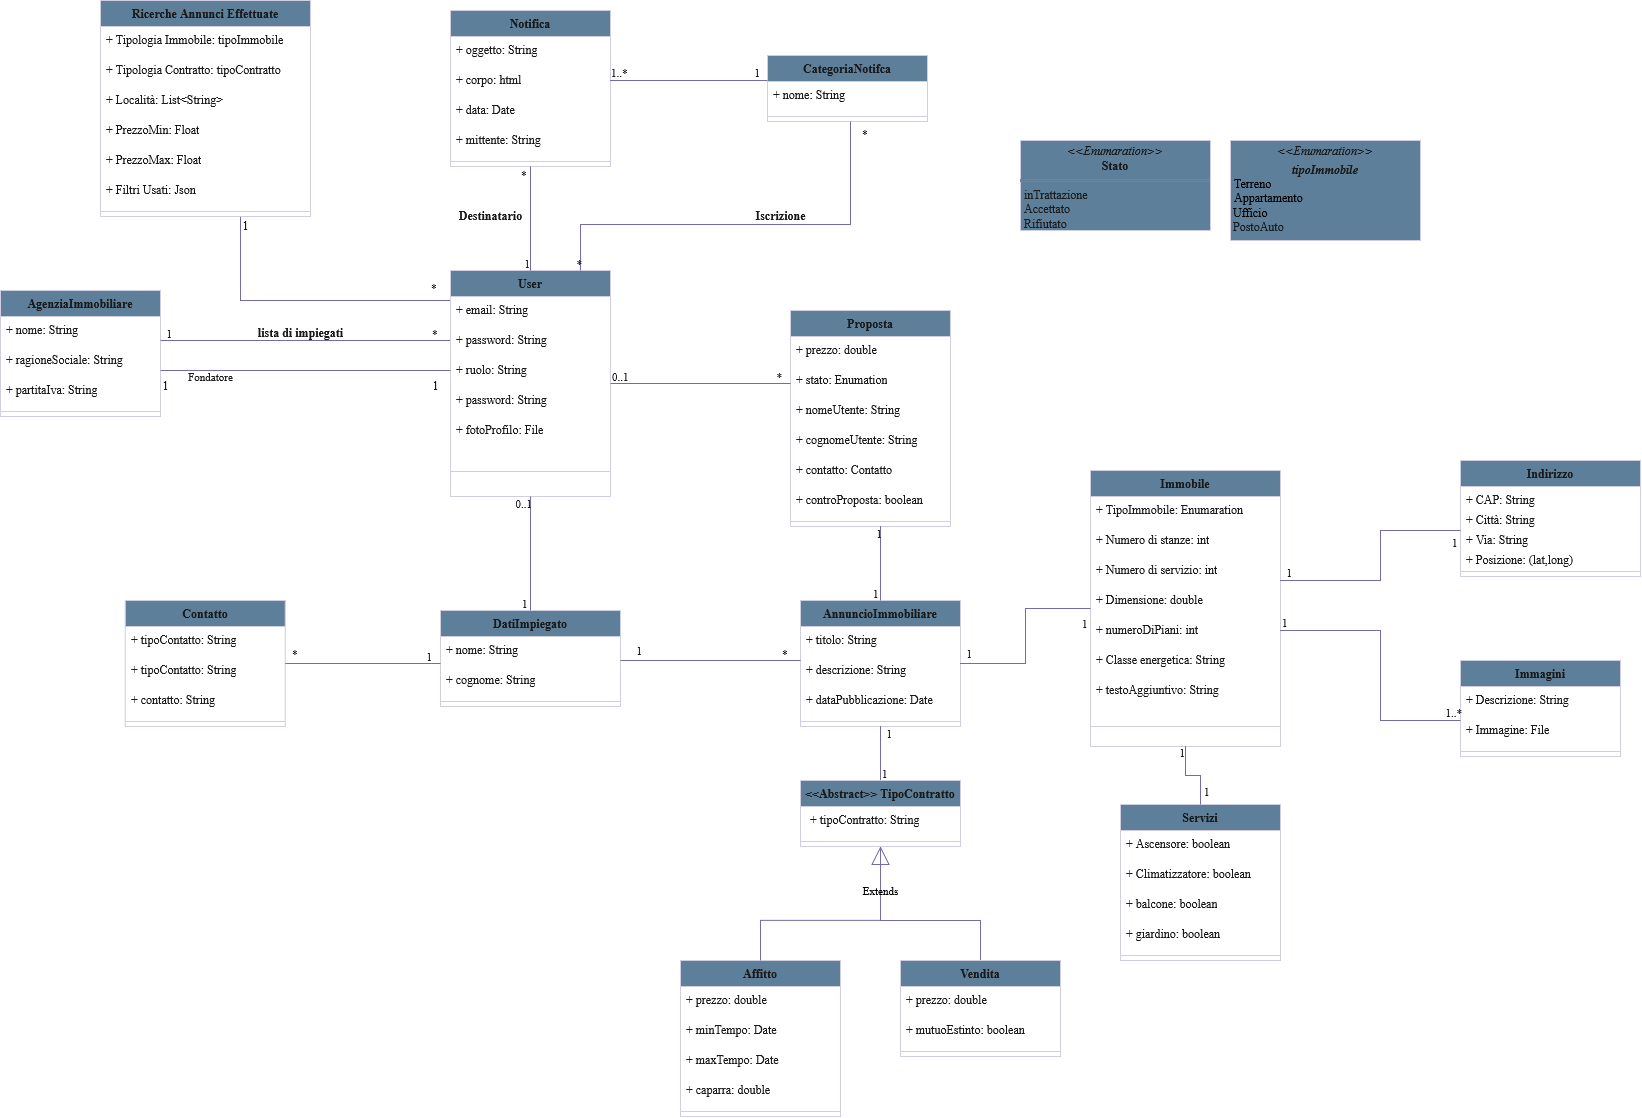
\includegraphics[width=1
    \linewidth]{Immagini/diagramma delle classi.drawio.png}
    \caption{Diagramma delle classi usate}
    \label{fig:enter-label}
\end{figure}
